\chapter{实验分析}
本文基于第三章里所提及的 ZORE 系统来进行中文文本的关系抽取。当中包括了 ZORE 在试验的语料库上的运行及其抽取关系实验。本章首先介绍了当前主流的对于开放式关系抽取算法评价指标,之后介绍了如何获取对当前算法评估所需的数据以及将 ZORE 算法与 DPM 算法进行对比,列出并分析了实验结果以及实验中出现的错误出现原因,提出基于实验数据的对 ZORE 进行性能提高设想。
\section{评判标准}对于 ZORE 系统的评判指标,此处使用主流论文对于开放式关系抽取算法的评价指标:准确率(Precision)、召回率(Recall)、综合评价 F1 值。

为了精确地统计 ZORE 系统运行关系抽取功能于各语料库内的性能数据,采用人工对抽取结果进行检查。实验数据的统计方法为:第一步,对 ZORE 算法的抽取结果进行人工标注,判断其求出的关系元组是否符合人的理解方式,若符合,则将该组标注为 $True$,反之则标注为 $False$,$T$ 为全部的有 $True$ 标记的关系元组集,$N$ 则为全部的有 $False$ 标记的关系元组集,$A$ 表示所有被抽取出的关系元组集,$A=T\cup N$。$S$ 则表示人工对语料库标注的实际正确关系集合。
    \begin{equation}
        Precision=\frac{|T|}{|A|}\times 100\%
    \end{equation}
    \begin{equation}
        Recall=\frac{|T|}{|S|}\times 100\%
    \end{equation}
    \begin{equation}
        F1=\frac{2\times Precision\times Recall}{Precision+Recall}
    \end{equation}

显然,Precision 为算法所求得的正确关系元组数占所有关系元组的百分比,算法抽取的关系的正确结果比例随着 Precision 的升高而升高。召回率则表示算法所求出的正确关系占实际正确关系的比例,可以提供算法抽取关系是否全面的评价指标,随着比例增高遗漏实际正确关系的概率会降低。普遍状态下,召回率与精确率成反比,即召回率越高精确率越低,故还有指标 F1 来评价算法的综合性能,显然,F1 越大则算法全面表现越出色。

\section{实验环境构建}
操作系统:Windows10,java version 1.8.0\_131,IDE 使用 Eclipse。在语料库“燃规3”中运行 ZORE。本语料库经过过滤“燃规3” ~\citep{rangui3} 中未以标点符号结尾的句子后,由 331 个句子构成,而中文词典《同义词林》\citep{che2005}则被用来提供每个字词的语义类别。《同义词林》包含了 77492 个中文字词,并被组织为五级的分层。在顶层有 12 个类别,第二、第三层则分别有 94 和 1492 个类别。在 ZORE 系统中以第二层的类别作为语义分类基准。而模式匹配的阈值 $t^{lvc}$ 与 $t^{sem}$ 分别设置为 0.4 与 3。

对于实验文本的数据集,因为是法规类文本,所以需要对每个条目开头的数字编号进行处理,以避免进行关系抽取时这些数字对关系抽取产生影响。因为每个条目开头数字编号的结构是“数字.数字.数字”,即 python 下的正则表达式类型为 $\backslash d\backslash .\backslash d\backslash .\backslash d$。以下为 python 对文本数据的预处理:

\begin{lstlisting}[language=python, caption=python 文本预处理, label={code:pythonpreprocess}]
import re

fo = open("foo.txt", "r")
bar = open("foo_modified.txt", "w")
while 1:
    line = fo.readline()
    if not line:
        break
    line = re.sub("\d\.\d\.\d", "", line)
    bar.write(line)
fo.close()
bar.close()
\end{lstlisting}

对输入文本进行完去除噪声处理之后,便可以开始使用 ZORE 对文本进行处理。处理完成后,ZORE 将文本中抽取出的关系以 $*.xml$ 的方式进行存储,图 ~\ref{fig:result} 表示了 ZORE 从“燃规3”中的一个句子里提取出的关系。

输出的关系文件当中存在 ZPar 依存分析的标签,各标签的含义如表 ~\ref{tab:ZParDep}。

\begin{longtable}{|c|c|c|c|}
% 首页表头
\caption[ZPar 依存分析标签]{ZPar 依存分析的标签} \label{tab:ZParDep} \\
\toprule[1.5pt]
 标签 & 含义 & 标签 & 含义 \\
\midrule[1pt]
\endfirsthead
% 续页表头
\caption[]{ZPar 依存分析的标签(续)} \\
\toprule[1.5pt]
 标签 & 含义 & 标签 & 含义 \\
\midrule[1pt]
\endhead
% 首页表尾
\hline
\multicolumn{4}{r}{\small 续下页}
\endfoot
% 续页表尾
\bottomrule[1.5pt]
\endlastfoot
    ROOT    &   核心关系    &  VOB     &   动宾关系    \\
    \hline
    RAD     &   右附加关系    & RED    &   重复元素    \\
    \hline
    SBV     &   主谓关系     & RADC    &   非共享右附加关系    \\
    \hline
    PUS     &   句中标点      & IOB    &   间宾关系    \\
    \hline
    POB    &   介词宾语      & ACT    &   动词性宾语    \\
    \hline
    ATT    &   定中关系     & ADV    &   状中关系    \\
    \hline
    CMP    &   动补关系      & APP    &   同位语关系    \\
    \hline
    COO    &   并列关系      & COS    &   右共享并列关系    \\
    \hline
    IC    &   独立子句     & IS    &   独立结构    \\
    \hline
    PUN    &   句末标点      &  TPC    &   主题    \\
    \hline
    VV    &   串行动词      & MT    &   时态    \\
    \hline
    NUM    &   数量      & QUN    &   度量关系    \\
    \hline
    QUC    &   前置量词     & QUCC    &   非共享前置量词    \\
    \hline
     ISC    &   非共享独立结构      & LAD    &   左附加关系    \\
\end{longtable}

因为 ZORE 利用 ZPar 进行依存句法分析,所以输出的关系文件当中存在 ZPar 所定义的词性标注的标签,各标签的含义如表 ~\ref{tab:ZParSem}。

\begin{figure}[htb]
\centering
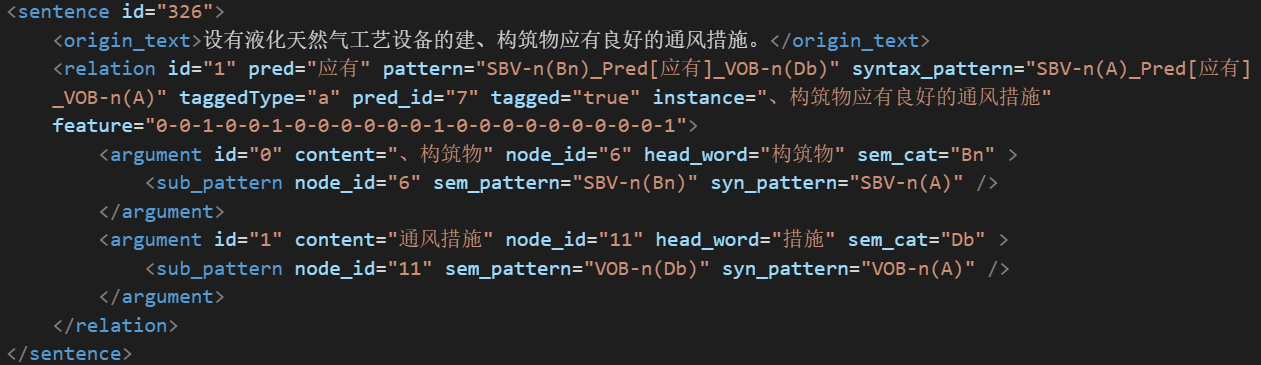
\includegraphics[width=15cm]{result}
\caption{ZORE 的输出}\label{fig:result}
\end{figure}

\begin{longtable}{|c|c|c|c|}
% 首页表头
\caption[ZPar 词性标注标签]{ZPar 词性标注的标签} \label{tab:ZParSem} \\
\toprule[1.5pt]
 标签 & 含义 & 标签 & 含义 \\
\midrule[1pt]
\endfirsthead
% 续页表头
\caption[]{ZPar 词性标注的标签(续)} \\
\toprule[1.5pt]
 标签 & 含义 & 标签 & 含义 \\
\midrule[1pt]
\endhead
% 首页表尾
\hline
\multicolumn{4}{r}{\small 续下页}
\endfoot
% 续页表尾
\bottomrule[1.5pt]
\endlastfoot
    a    &   形容词    &  d     &   副词    \\
    \hline
    c     &   连词    & e    &   感叹词    \\
    \hline
    f     &   方位词     & o    &   拟声词    \\
    \hline
    g     &   语素词      & h    &   前缀成分    \\
    \hline
    i    &   成语      & p    &   介词    \\
    \hline
    q    &   量词     & s    &   所处词    \\
    \hline
    y    &   语气词      & t    &   时间词    \\
    \hline
    v    &   动词       & nrf    &   姓氏    \\
    \hline
    nx    &   非汉语名词     & b    &   区别词    \\
    \hline
    m    &   数词      &  j    &   简称缩写    \\
    \hline
    k    &   后缀成分      & l    &   习语    \\
    \hline
    n    &   名词      & nr    &   人名    \\
    \hline
    ns    &   地名     & nt    &   机构团体    \\
    \hline
     nz    &   其他专名词      & r    &   代词    \\
    \hline
     x    &   非语素词      & z    &   状态形容词    \\
    \hline
     u    &   助词      & w    &   标点    \\
    \hline
     nrg    &   姓      &     &       \\
\end{longtable}

% 而关系(taggedType)则有“a,n,h,t”四种,分别代表“默认的被抽取出的关系,通过相关关系标注,未被标注且已知语义模式,已被标注且已知语义模式”。
feature 为类似于表 ~\ref{tab:feature} 中的对应 feature 的符合关系,其中增加了对于四种 taggedType 的判断,以“1”为符合条件,“0”不符合条件来进行标注。以图 ~\ref{fig:result} 作为句子抽取实例,可以读出,这个句子为语料库中第 326 个句子(sentence id = 326),仅被抽取出一个关系,关系类型为普通,谓词是“应有”(pred = “应有”),语义模式为\{ SBV-n(Bn),Pred[应有],VOB-n(Db) \},查表 ~\ref{tab:ZParDep} 可得前后两个论元的依存类型分别为主谓关系(SBV)和动宾关系(VOB),谓词是句子里从左到右的第七个词汇,语法模式为\{ SBV-n(A),Pred[应有],VOB-n(A) \}。在两个论元里,则提供了其在依存树中的节点序号、核心词汇、内容以及语义类型(sem\_cat),还有其子模式的具体信息。

还可以发现其对语句里关系的抽取遗漏了一个关系(设有液化天然气工艺设备,的,建、构筑物),所以 ZORE 算法对于中文文本的开放式关系抽取并不是完全覆盖的,也就涉及到了下文对于 ZORE 算法的评价以及获取全面、正确的手工标注关系数据集所需要做的工作。

\section{实验结果分析与评价}
本文对被提取出的关系的精确度(Precision)和召回率(Recall)进行评价。一个被提取出的关系仅在谓词短语和其他的所有论元匹配了全部的句中内容才被认为是正确的、有意义的。

对语料库“燃规3”进行中文开放式关系抽取耗费的总时间虽然较长,但其包括读取知识库和对中文语料库进行自然语言处理的 203 秒和对文本进行解析的接近一分钟的时间,可见该系统的运行效率很大程度上受到对中文语料库进行自然语言处理效率不是很高的拖累。可以考虑换用其他类型的自然语言处理工具来替代当前 ZORE 系统中的 StanFord NLP 自然语言处理模块从而帮助提升系统的整体效率。

以人工标注的“燃规3”关系文件 relation-500-human.xml 作为实际正确关系集 $S$,relation-500.xml 作为算法提取出的关系集 $A$,语义模式重复频度阈值的初始值设为 19,以 1 为步长递减至 3,以下为评价程序的工作代码,本程序源代码及人工标注的关系文件上传于 https://github.com/zaynr/GraduationThesis。

\begin{lstlisting}[language=java, caption=评价程序, breaklines=true, label={code:evaluate}]
public static void main(String[]args){
    for(int i=19;i>3;i--){
        EvaluateCORE evaluate=new EvaluateCORE();
        String sHumanTaggedFileName="tagged/relation-500-human.xml";
        String sAutoTaggedFileName="result_origin_rule/relation-500.txt";
        String sOutputFileName="score.txt";
        evaluate.nThresholdSem=i;
        evaluate.filterType="tn";
        System.out.println("evaluate.filterType="+evaluate.filterType);
        String sPatterFileName="result_origin_rule/pattern_synset.txt";
        evaluate.readPatternScore(sPatterFileName,"gbk");
        evaluate.evaluate(sHumanTaggedFileName, sAutoTaggedFileName,sOutputFileName);
    }
}
\end{lstlisting}

其中,evaluate(String sHumanTaggedFileName, String sAutoTaggedFileName, String sOutputFileName) 这个函数是这个评价程序的核心,对 ZORE 输出的关系抽取结果 $sAutoTaggedFileName$ 与人工标注的关系文件 $sHumanTaggedFileName$ 进行比较,$sOutputFileName$ 则记录了了输出的比较数据记录。

对人工标注的关系文件与 ZORE 算法生成的关系文件当中句子逐个按照关系、论元、谓词短语进行比较,此函数调用了 compareTwo(Vector<ExtractedSentence> vecHumanSentence, Vector<ExtractedSentence> vecAutoSentence)。

比较的思想为,首先尝试将人工标注关系与 ZORE 提取出的关系的谓词短语进行匹配测试,若匹配成功则继续进行二者的论元匹配测试;若至少存在一个论元匹配,则自增谓词短语正确数,若所有论元都匹配成功,则自增关系正确数;之后往论元正确数加上当前匹配成功的论元个数,经过以上的处理之后,就得出了计算精确率 Precision 所需的“正确关系数”与“总关系数”。

因为考虑到当前 ZORE 系统所调用的自然语言处理模块不能很好地将以“的”和“是”作为谓词短语的向心结构关系进行分词、依存分析、词性标注,故会影响到 ZORE 系统对其的抽取,这并不是由于 ZORE 算法设计失误导致的抽取缺陷,并且以“的”和“是”作为谓词短语的向心结构关系经过训练集训练之后已经得出是一种高频出现的关系,如果将其包括在内会影响召回率的计算,所以对于召回率 Recall 计算时,人工标注的关系集 $S$ 将以“的”和“是”作为谓词短语的向心结构关系排除在外。

对于语料库的手工标注关系数据集,基于 ZORE 算法所输出的三千多行关系集文件“relation.xml”进行修改。因为评价程序对于关系的评价数据的精确率 Precision 、召回率 Recall 以及由前二者计算出的 F1 值只是基于评价程序中对于谓词短语 predicate、谓词短语的论元内容 arguArr.content 和手工标注关系数据集与 ZORE 生成的关系集文件的二者对应的关系的论元个数 arguArr.size() 来进行匹配。所以在手工标注时无视其他在 ZORE 算法所输出的关系集文件内关系的其他参数,仅仅关注于四个方面:第一,语句当中含有的关系数量,由其 relation id 体现;第二,关系集当中的谓词短语 predicate phrase 是否正确;第三,关系中的论元内容 content 是否正确;第四,关系中的论元个数是否正确。进行多个独立专家标注关系数据集并将其用交叉对比形式保证准确客观性的成本极高,而自己动手进行标注的话可以加深对于自然语言处理及其关系抽取的理解,所以本次进行实验的对 ZORE 输出手工标注关系数据集由作者进行,尽力以客观、简洁的方式审阅 ZORE 算法输出的数据集文件并进行人工标注,从而获得评价 ZORE 算法所需的手工标注关系数据集文件“relation-500-human.xml”。

\begin{longtable}{|c|c|c|c|}
% 首页表头
\caption[ZORE 性能数据]{ZORE 运行于语料库“燃规3”上的性能数据} \label{tab:ZOREperformance} \\
\toprule[1.5pt]
 召回率 & F1 值 & 精确率 & $t^{sem}$\\
\midrule[1pt]
\endfirsthead
% 续页表头
\caption[]{ZORE 运行于语料库“燃规3”上的性能数据(续)} \\
\toprule[1.5pt]
 召回率 & F1 值 & 精确率 & $t^{sem}$\\
\midrule[1pt]
\endhead
% 首页表尾
\hline
\multicolumn{4}{r}{\small 续下页}
\endfoot
% 续页表尾
\bottomrule[1.5pt]
\endlastfoot
0	&	0	&	1	&	19\\
    \hline
0.02	&	0.039111111	&	0.88	&	18\\
    \hline
0.05	&	0.094117647	&	0.8	&	17\\
    \hline
0.1	&	0.178494624	&	0.83	&	16\\
    \hline
0.14	&	0.24040404	&	0.85	&	15\\
    \hline
0.2	&	0.323809524	&	0.85	&	14\\
    \hline
0.245	&	0.383288889	&	0.88	&	13\\
    \hline
0.294	&	0.435555556	&	0.84	&	12\\
    \hline
0.343	&	0.483680138	&	0.82	&	11\\
    \hline
0.392	&	0.526174497	&	0.8	&	10\\
    \hline
0.4394	&	0.562132196	&	0.78	&	9\\
    \hline
0.4532	&	0.565559907	&	0.752	&	8\\
    \hline
0.4743	&	0.574383099	&	0.728	&	7\\
    \hline
0.4876	&	0.557208158	&	0.65	&	6\\
    \hline
0.5358	&	0.576546301	&	0.624	&	5\\
    \hline
0.5674	&	0.574899548	&	0.5826	&	4\\
    \hline
0.6193	&	0.545454545	&	0.512	&	3\\
\end{longtable}

\begin{figure}[t]
\centering
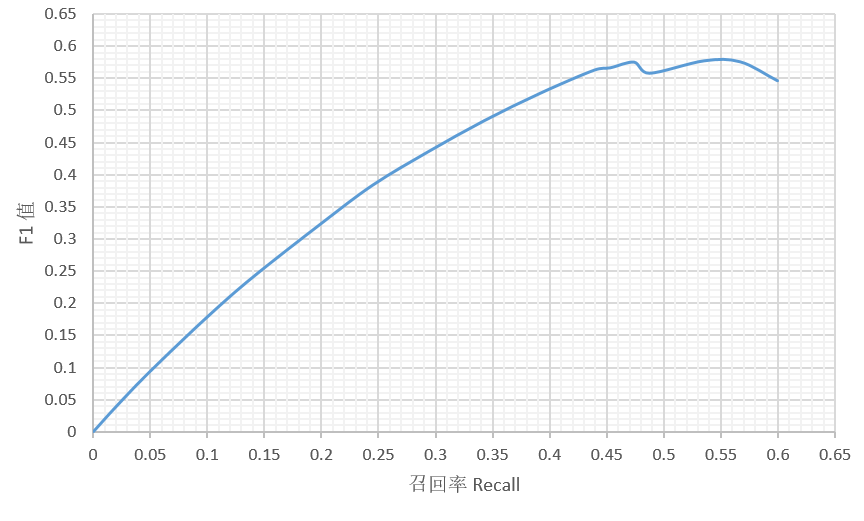
\includegraphics[width=15cm]{performance}
\caption[ZORE 性能图]{ZORE 基于语料库“燃规3”的 F1 值}\label{fig:performance}
\end{figure}

评价程序数据生成的算法性能图 ~\ref{fig:performance} 以 F1 值作为 ZORE 算法综合性能的评价,下表为基于运行评价程序所得出的数据。可以看出,随着词性过滤阈值 $t^{sem}$ 的下降,算法的召回率 Recall 不断提高,而精确率 Precision 却在不断下降,对算法的综合性能衡量指标 F1 值则上下浮动,大体上呈现一种多次函数的模式。

图 ~\ref{fig:performance} 显示了在不同的召回率下 ZORE 在“燃规3”数据集中的表现。体现了先前提及的对召回率 Recall 与精确度 Precision 的平衡性权衡,即 F1 的值先是随着召回率 Recall 的增加而增加,到达极大值后开始下降,则选择 F1 拥有极大值处的召回率 Recall 值可以获得当前语料库下 ZORE 算法的最佳综合性能表现。

同时,以另一种开放式关系抽取算法 DPM\citep{liyang2016} 来与 ZORE 的性能进行比较。二者之间最大的区别就是 DPM 算法增加了对于兼类词的探测和处理,使词性标注出现错误的概率降低,从而提升关系抽取的精确性 Precision,其余处理部分大体相同,也可称之为 ZORE 的兼类词处理版本。

\begin{figure}[h!]
\centering
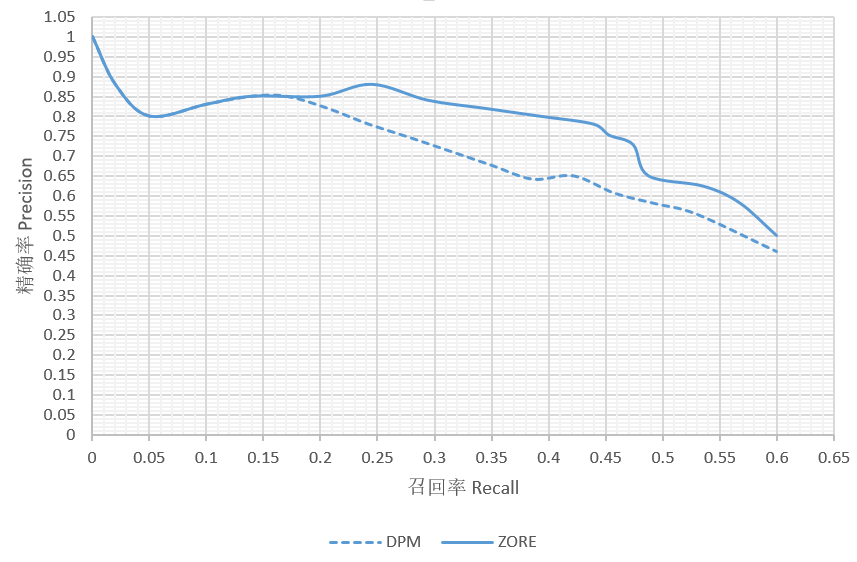
\includegraphics[width=15cm]{compare}
\caption{ZORE 与 DPM 的 P-R 曲线对比}\label{fig:compare}
\end{figure}

\begin{longtable}{|c|c|c|c|}
% 首页表头
\caption[DPM 性能数据]{DPM 运行于语料库“燃规3”上的性能数据} \label{tab:DPMperformance} \\
\toprule[1.5pt]
 召回率 & F1 值 & 精确率 & $t^{sem}$\\
\midrule[1pt]
\endfirsthead
% 续页表头
\caption[]{DPM 运行于语料库“燃规3”上的性能数据(续)} \\
\toprule[1.5pt]
 召回率 & F1 值 & 精确率 & $t^{sem}$\\
\midrule[1pt]
\endhead
% 首页表尾
\hline
\multicolumn{4}{r}{\small 续下页}
\endfoot
% 续页表尾
\bottomrule[1.5pt]
\endlastfoot
0	&	0	&	1	&	19\\
\hline
0.02	&	0.039111111	&	0.88	&	18\\
\hline
0.05	&	0.094117647	&	0.8	&	17\\
\hline
0.1	&	0.178494624	&	0.83	&	16\\
\hline
0.14	&	0.24040404	&	0.85	&	15\\
\hline
0.17	&	0.283333333	&	0.85	&	14\\
\hline
0.206	&	0.329278752	&	0.82	&	13\\
\hline
0.242	&	0.369393346	&	0.78	&	12\\
\hline
0.278	&	0.405152895	&	0.746666667	&	11\\
\hline
0.314	&	0.435742606	&	0.711666667	&	10\\
\hline
0.35	&	0.461363636	&	0.676666667	&	9\\
\hline
0.386	&	0.48203049	&	0.641666667	&	8\\
\hline
0.422	&	0.511753731	&	0.65	&	7\\
\hline
0.458	&	0.521830254	&	0.606333333	&	6\\
\hline
0.494	&	0.533556797	&	0.58	&	5\\
\hline
0.53	&	0.5415749	&	0.553666667	&	4\\
\hline
0.5931	&	0.520754717	&	0.464	&	3\\
\end{longtable}

\begin{figure}[h!]
\centering
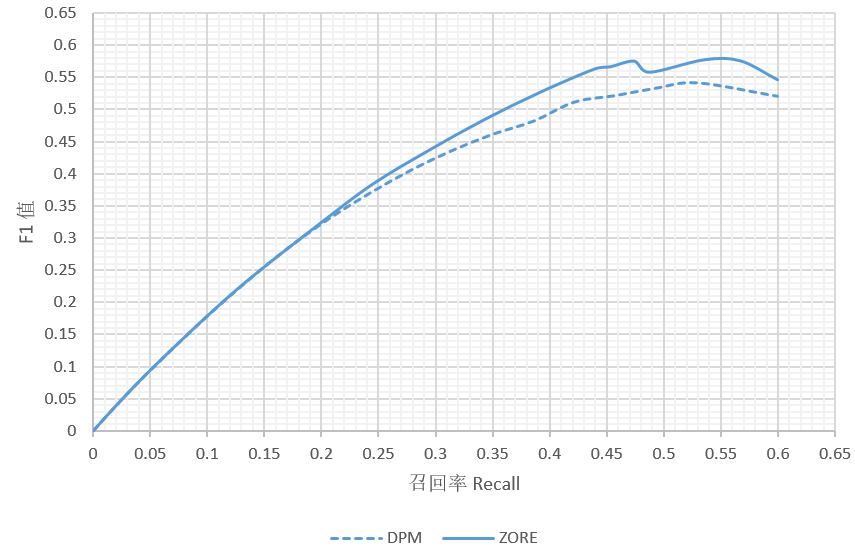
\includegraphics[width=15cm]{comparef}
\caption{ZORE 与 DPM 的 F1 值对比}\label{fig:comparef}
\end{figure}

为了对比的公正客观性,也以“燃规3”作为其语料库进行处理。图 ~\ref{fig:compare} 即为二者运行于同一语料库上的对比图表,可见在特定召回率 Recall 区间上,DPM 精确度 Precision 劣于 ZORE 算法,推断是是由于该语料库是法规,文本结构较为碎片化,以上下文环境进行分析的兼类词处理难以顺利工作导致的。

二者的 P-R 曲线都是体现了精确率 Precision 与召回率 Recall 成反比关系。以及二者之间 F1 值在各种召回率 Recall 下的表现,如图 ~\ref{fig:comparef} 所示,可以看出 DPM 与 ZORE 之间的 F1 值区别并不大,所以可以推断,仅仅增加了对于兼类词处理模块的改进 ZORE 算法得到的 DPM 并没有本质上的提升,即缺少对兼类词处理不是 ZORE 算法提升性能所遇到的瓶颈。

本文经过 ZORE 对语料库“燃规3”进行关系抽取之后,得到了“type\_new.txt”这个所提取出的关系模式统计文件,当中包括了 30 个关系模式及其在训练数据集当中出现的频次和在当前所处理的语料库中出现的频次,以 20 次作为高频出现的阈值,这 30 个关系模式中存在 3 个高频关系模式,分别为:Pattern(nsubj-m(Dn), Pred[de], dobj-n(Di)),22 次;Pattern(nsubj-n(A0), Pred[de], dobj-n(A1)),38 次;Pattern(nsubj-q(Dn), Pred[de], dobj-n(Di)),21 次。很显然,这三个模式都是以“的”为谓词短语的关系模式,与现实生活里的经验符合:由“的”构成的三元组关系模式占正常生活里中文语境下的文本的大多数。

\section{错误分析}
在观察了输出的结果文件后,对不正确的提取(由于精确度的损失)与遗漏的正确的关系(由于召回的损失)进行了统计,得出约 $40\%$ 的遗漏关系是因为语义模式的最低频率限制所导致,而对于语义模式最低频率的限制则是用来平衡召回率与精确率的。

还有一个主要的错误原因是由于解析错误导致的对谓词短语的错误鉴别,带来了全部错误中约 $37\%$ 的报错。也存在由于自然语言处理工具所导致的错误,有分词、依存句法、词性标记等方面产生的错误,例如图 ~\ref{fig:result} 中 argument id = 0 的论元应为 “建、构筑物”而不是“、构筑物”。

这个分词错误也导致了 ZORE 对 id = 326 的句子进行关系抽取时产生了遗漏,关系(设有液化天然气工艺设备,的,建、构筑物)应该在分词正确的前提下被抽取出来。分词错误还会导致对论元的归纳错误,进而影响对 feature 匹配的计量,无法对当前进行分析的句子通过所符合的 feature 数量进行正确的置信度计算,最终影响关系的置信度权重值,使 $Logistic$ 回归分类器无法以当初所预计的工作效果继续工作。

在进行关系提取的过程中也存在选择了错误的模式进行抽取以及未找到可以进行匹配的模式的问题,举个例子,“为使城镇燃气工程设计符合安全生产、保证供应、经济合理和保护环境的要求,制定本规范。”这个句子就未搜索到可以和他匹配的模式进行关系抽取,进而遗漏了(使城镇燃气工程设计,符合,安全生产、保证供应、经济合理和保护环境的要求,制定,本规范),(安全生产、保证供应、经济合理和保护环境,的,要求)这两个关系。

分析结果表明,ZORE 的提取所得到的模式精确率与全面率还有待提升,另外,经过分析可以得出:自然语言处理的工具的性能是提升开放式关系提取算法的瓶颈,句法分析的提升和更加全面且精确的分词系统有很大的可能性让开放式关系抽取也随之进步,所以进行深入研究关于自然语言的处理也是提升开放式关系抽取系统效率的方法之一。亦可追加关系元组进入关系知识库当中,以增加匹配面,故也可对知识库的应用加以研究。

\section{本章小结}
这一章完成了基于特定语料库的算法运行,并对算法的运行结果进行了分析,根据经典的对开放式关系抽取系统的评价标准 P-R 图衡量了算法 ZORE 的综合性能,并验证了词性标签阈值 $t^{sem}$ 对 P-R 图的影响、P-R 二者之间成反比的关系与其权衡。

将 ZORE 与其拥有兼类词处理版本的算法 DPM 进行对比,分析并得出了兼类词处理对于中文开放式关系抽取系统的精确率 Precision 的影响推论。

对于 ZORE 系统的改进,提出了加强系统所使用自然语言处理模块的性能,包括其分词、词性标注、依存句法分析的准确性提高;向关系知识库中追加新的关系元组以增大匹配面;添加对模式进行筛选的算法从而提高对其鉴别的准确性和其对语料库的覆盖率等未来研究方向的设想。